\documentclass{article}
\usepackage[UTF8]{ctex}
\usepackage{geometry}
\geometry{a4paper,left=1cm,right=1cm,top=1.5cm,bottom=2cm}
\usepackage{amsmath}
\usepackage{booktabs}
\usepackage{amsfonts}
\usepackage{graphicx}
\usepackage{float}
\usepackage[utf8]{inputenc}
\usepackage[T1]{fontenc}
\begin{document}
\title{\textbf{Logistic Regression}}
\maketitle
\centerline{\author{Huacheng Li}}
\begin{abstract}
    NCE的作用就是
\end{abstract}

\begin{table}[H]
    \centering
    \begin{tabular}{p{3cm} p{9cm}}
        \toprule
        \textbf{Symbols} & \textbf{Descriptions} \\ \midrule
        $x^i \in \mathbb{R}^d$ & 样本$x^i$的$d$维特征向量 \\ 
        $\theta=\{W^T, b\}$ & 模型的参数 \\ 
        $\hat{y}^i \in \mathbb{R}^1$ & 样本$x^i$对应的预测输出\\ 
        $Y^i \in \mathbb{R}^1$ & 样本$x^i$对应的真实标签\\ 
        $m$ & 样本个数 \\
        \bottomrule
        
    \end{tabular}
\end{table}


\section{Logistic分布}

如图\ref{FIG:LogisticDist}所示,Logistic分布是一种连续型概率分布,其分布函数$F(x)$和密度函数$f(x)$如下所示。
\begin{equation}
    \begin{split}
        F(x) = P(X \le x) = \frac{1}{1+e^{-(x-\mu)\gamma}} \\
        f(x) = F^{'}(x) =\frac{e^{-(x-\mu)\gamma}}{\gamma (1+ e^{-(x-\mu)\gamma})^2}
    \end{split}
\end{equation}

\begin{figure}[H]
    \centering
    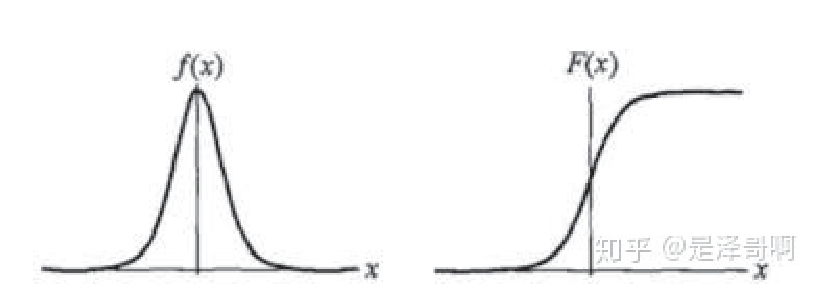
\includegraphics{graphics/LogisticDistribution.eps}
    \caption{Logistic分布}
    \label{FIG:LogisticDist}
\end{figure}

Sigmoid函数是$\mu=0, \gamma = 1$时的特例,其中$\mu$是位置参数,$\gamma$是形状参数。

\section{Logistic Regression 模型}

\subsection{模型方法}
Logistic Regression最早的文献已经不可考,目前找到的较早的文献是\cite{efron1975efficiency}。
Logistic Regression主要用于分类问题中。
以二分类为例,对于任意样本,我们首先将其表示为$d$维特征向量$x^i \in \mathbb{R}^d$。之后我们希望存在一个决策边界
\begin{equation}
    W^T x +b = 0
\end{equation}
能够对样本分类。即如果$W^T x^i+b>0$,那么该样本类别为1,否则为0。
而函数$l(x)=W^T x+b$取值是连续的,无法拟合离散变量$\{0,1\}$,可以基于它设计条件概率$p(Y=1|x)$,因为概率的取值也是连续的。
最理想的是阶跃函数
\begin{equation}
    p(Y = 1|x) = \begin{cases}
        0,& Wx+b<0\\
        0.5,& Wx+b=0\\
        1,& Wx+b>0
    \end{cases}
\end{equation}
但是阶跃函数不可微,因此考虑使用Sigmoid/Logistic函数将函数$h(x)$的值放缩到区间$\left[0,1\right]$。

\begin{equation}
    P(Y=1|x) = \sigma(W^T x+b) = \frac{1}{1+e^{-(W^T x+b)}}
    \label{EQU:LogisticRegression}
\end{equation}

因此,$l(x) = W^T x +b$为线性回归,加入Sigmoid/Logistic函数后变为Logistic回归。
为了表示方便,我们可以用参数$\theta$表示模型中的所有参数。
这样一来,对于样本$x^i$,我们可以根据预测结果做出分类:
\begin{equation}
    \tilde{y}^i = \begin{cases}
        0,& \sigma(\theta x^i) <0.5 \\
        1,& \sigma(\theta x^i)\ge 0.5
    \end{cases}
\end{equation}


\subsection{对数几率}
公式 (\ref{EQU:LogisticRegression})可以重写为
\begin{equation}
    \ln \frac{y}{1-y} = \theta x = W^T x + b
\end{equation}
其中$\frac{y}{1-y}$被称为odds(几率),它反映了样本$x$作为正例的相对可能性。
对对数求几率,也被称为``对数几率''(log odds,亦称logit)。
由于希望能够使用形容词来修饰Regression,因此被称为Logistic Regression。这个和中文中的逻辑没有关系。

\subsection{优势}
\begin{itemize}
    \item 直接对分类的概率进行建模,无需假设数据分布,从而避免了假设分布不准确带来的问题(区别于生成式模型)
    \item 不仅可以预测出类型,还能得到预测的概率。这对于一些利用概率辅助决策的任务很有用
    \item 对数几率函数是任意阶可导的凸函数,许多数值优化算法都可以求解。
\end{itemize}

\section{损失函数}

\subsection{MLE}
Logistic Regression的损失函数是根据极大似然估计思想来设计的。
对于二分类问题,我们可以将其输出概率重写为
\begin{equation}
    P(\hat{y}^i = Y^i | X^i) = \begin{cases}
        \sigma(\theta x^i),& Y^i=1,\text{即样本$x^i$实际标签为1}\\
        1-\sigma(\theta x^i),& Y^i = 0, \text{即样本$x^i$实际标签为0}
    \end{cases}
\end{equation}

如果模型输出$P(x^i)$的值在0.5附近,那么分类既像1,又像0。说明分类恨不准确,没有意义。
为了分类准确,我们希望标签为0和1的样本的预测输出尽可能不一样。

\textbf{模型的预测结果由模型参数$\theta$决定,而参数$\theta$是由数据集训练而来的。为了能够使预测结果和真实标签一致,对于每个样本$x^i$,我们可以构建如公式(\ref{EQU:SampleUnitedProbability})似然函数。}

\begin{equation}
    P(\hat{y}^i = Y^i | x^i) = (\sigma(\theta x^i))^{Y^i} \star (1-\sigma(\theta x^i))^{1-Y^i}
    \label{EQU:SampleUnitedProbability}
\end{equation}

\textbf{为了能够使模型训练的更好,我们希望在训练数据上,模型的预测结果和真实结果的差距尽可能的小,因此我们可以构建所有样本的损失函数,如公式(\ref{EQU:MLEProd})所示。}
\begin{equation}
    \mathcal{L}(\theta) = \prod^m_{i=1} P(\hat{y}^i = Y^i |x^i)=\prod^m_{i=1} (\sigma(\theta x^i))^{Y^i} \star (1-\sigma(\theta x^i))^{1-Y^i}
    \label{EQU:MLEProd}
\end{equation}

我们希望使$\mathcal{L}(\theta)$最大化。因为$\mathcal{L}(\theta)$表示模型预测输出与真实值的相似度,越相似,$\mathcal{L}(\theta)$越大。因此 最大化$\mathcal{L}(\theta)$相当于找到性能最好的模型,找到最好的$\theta^{*}$。且最大化$\mathcal{L}(\theta)$和最大化$\log \mathcal{L}(\theta)$等价。

\begin{equation}
    \log \mathcal{L}(\theta) = \sum^m_{i=1} \left[ Y^i \star \log \sigma(\theta x^i) + (1-Y^i) \star \log (1-\sigma(\theta x^i))  \right]
    \label{EQU:MLESum}
\end{equation}

\subsection{Loss函数}

我们将损失函数定义如下。


\begin{equation}
    logloss \mathcal{L}(\theta) = -\frac{1}{m} \star \sum^m_{i=1} \left[ Y^i \star \log \sigma(\theta x^i) + (1-Y^i) \star \log (1-\sigma(\theta x^i))  \right]
    \label{EQU:LogLoss}
\end{equation}

相比于公式(\ref{EQU:MLESum})$\log \mathcal{L}(\theta)$,$logloss \mathcal{L}(\theta)$的改动主要是乘以$-\frac{1}{m}$。这一方面是为了消除样本数量的影响,另一方面是为了将Loss值变为正值。下面论述该损失函数的合理性。

对于样本$x^i$,有以下几种情况:
\renewcommand{\labelitemi}{$\bullet$}
\renewcommand{\labelitemii}{$\diamond$}
\begin{itemize}
    \item $Y^i=1$:
    \begin{itemize}
        \item $\sigma(\theta x^i)$ 越靠近1,则$\log \sigma(\theta x^i)$越靠近0(负值)
        \item $\sigma(\theta x^i)$ 越靠近0,则$\log \sigma(\theta x^i)$越靠近负无穷
    \end{itemize}
    \item $Y^i=0$:
    \begin{itemize}
        \item $\sigma(\theta x^i)$ 越靠近1,则$\log (1- \sigma(\theta x^i))$越靠近负无穷
        \item $\sigma(\theta x^i)$ 越靠近0,则$\log (1- \sigma(\theta x^i))$越靠近0(负值)
    \end{itemize}
\end{itemize}
加上前面的负号,logloss的值为正值。那么也就意味着预测的越正确,logloss越小;预测的越错误,logloss的值越大。

\section{为什么将LogLoss和交叉熵等价?}
交叉熵刻画的是两个分部之间的距离。当其作为损失函数时,即实际输出(预测分布)与期望输出(数据分布)之间的差异。也就是两个概率分布越接近,交叉熵越小。

假设期望分布为$p(x)$,实际输出为$q(x)$。那么交叉熵可以写为:
\begin{equation}
    H(p,q) = -\sum_{x} p(x) \log q(x)
\end{equation}


\subsection{Application}
在实际学习任务中,$p(x)$对应着样本的Label的分布,一般是One-Hot分布。因此,无论是正确还是错误,我们都要将其转化为1才可以使用。

以二分类为例。
假定一共有两个样本$x^1$和$x^2$,它们一个类别为0,一个类别为1。我们将其分别转化为$\left[0,1\right]$和$\left[1,0\right]$。
对于期望输出为$\left[0,1\right]$而言,实际输出为$\left[0.1, 0.9\right]$和$\left[0.4, 0.6\right]$,它们对应的交叉熵分别为0.0457和0.2218。


因此多分类样本的交叉熵可以定义为
\begin{equation}
    \mathcal{J}(\theta) = -\frac{1}{m} \sum^m_{i=1} \sum^n_{k=1} y_k^i \log (\hat{y}_k^i)
\end{equation}
其中$m$表示样本数量,$n$表示分类类别。
\begin{equation}
    y_k^i = \begin{cases}
        1,& Label(x^i)=K(\text{表示分到了对应的类别}) \\
        0,& others
    \end{cases}
\end{equation}

\begin{equation}
    logloss \mathcal{L}(\theta) = -\frac{1}{m} \star \sum^m_{i=1} \left[ Y^i \star \log \sigma(\theta x^i) + (1-Y^i) \star \log (1-\sigma(\theta x^i))  \right]
\end{equation}

根据上面的解释,我们可以看出,LogLoss实际上是类别为2的交叉熵损失函数。对于Label=1,直接是用标签$Y^i$。对于Label0,需要将其先转化为1,要使用$1-Y^i$作为$p(x)$

\bibliographystyle{apalike}
\bibliography{ref}

\end{document}